\documentclass[a4paper]{report}
%\addtolength{\oddsidemargin}{-.875in}
%\addtolength{\evensidemargin}{-.875in}
%\addtolength{\textwidth}{1.75in}
%\addtolength{\topmargin}{-.875in}
%\addtolength{\textheight}{1.75in}
\usepackage{amsmath} 
\usepackage{graphicx}
%\usepackage{geometry}
%\geometry{a4paper, top=3cm, bottom=3cm, left=3.5cm, right=3.5cm}
\DeclareUnicodeCharacter{2212}{-}
\title{DDPG + HER in FetchPush-v1 Gym Environment with Python3 and Tensorflow 2.0}
\author{Simone De Angelis 1760464\\ Veronica Romano 1580844}
\date{\today}


\begin{document}

\maketitle
\tableofcontents

\begin{abstract}
The purpose of this report will be to reproduce the results obtained in \cite{her} on a specific environment among the many presented in \cite{her}. First of all, we expose how the environment is represented and how our algorithm interacts with it. After that we highlight the differences between Deep Q-learning and Deep Deterministic Policy Gradient, focusing  on the general principles of DDPG combined with Hindsight Experience Replay.
The second part of the paper shows the results obtained following the same training procedure exposed in \cite{her} and a diffent one that will be explained in the corresponding section.
\end{abstract}
\chapter{Introduction and Work Purposes}
Reinforcement Learning is learning what to do and how to map situations to actions. The end result is to maximize the numerical reward. The learner is not told which action to take, but instead must discover which action will yield the maximum reward. As illustrated in Figure \ref{Fig: scheme}, an agent starts from a state $s_t$ and by choosing actions $a_t$ according to  a certain policy $\pi$ interacts with the environment that gives back to it  a reward $r_{t+1}$ and a new state $s_{t+1}$.

\begin{figure}[h!]
\centering
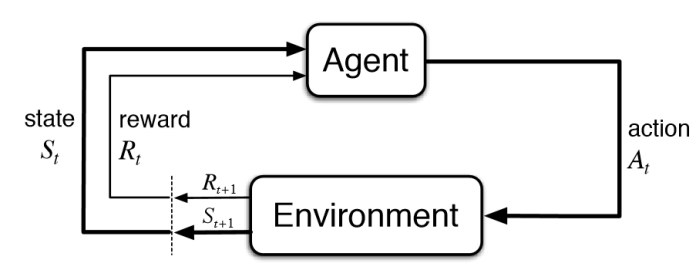
\includegraphics[scale=0.5]{reinforcement.jpg}
\caption{\label{Fig: scheme} Formulation of a basic Reinforcement Learning project.}
\end{figure}

This cycle proceeds until either a terminal condition or a goal is reached. 

\section{Environment and Tools}
We used OpenAI Gym environment combined with MuJoCo. In the past there weren't many standard environments that could be used to develop reinforcement learning algoirthms. In fact with the rise of OpenAi, reinforcement learning has become more practical and implementable with respect to previous  reinforcement learning methods. Gym is available on the corresponding GitHub repository and allows to use any of the environment present in the repository for free, from atari games to Robotic arms environemnt. The Fetch environment needs MuJoCo (Multi-Joint dynamics with Contact) that is an engine simulating real and detailed rigid body simulation with contacts forces. Mujoco-py is the library needed in order to work with tha gym environment, since it only supports python3 as programming language. However the best part is that MuJoCo provides the physical interactivity (like calculation of contact forces) which helps an engineer or researcher to test their model rigorously before moving to production.
\begin{figure}[h!]
\centering
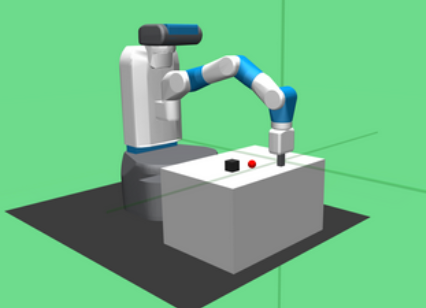
\includegraphics[scale=0.9]{fetchpush.png}
\caption{\label{Fig: fetchpush} FetchPush-v1 Gym environment.}
\end{figure}

The Fetch environment is based on the 7-DoF Fetch robotics arm which has a two-fingered parallel gripper that are locked to prevent grasping in the push task. The learned behavior is usually a mixture of pushing and rolling. The observation space is a dictionary object containing  
\begin{itemize}
\item observation: It's an array of 25 elements containing the cartesian position of the end effector, cartesian position and orientation of the desired object, its linear velocity as well as the position and linear velocity of the robot's gripper.
\item desired\_goal: The goal that the agent has to achieve. In FetchPush-v1 is the 3-dimensional target position on which we would like the box to be and it's represented by the red point in \ref{Fig: fetchpush}
\item achieved\_goal: The goal that the agent has currently achieved represented by the black box in figure \ref{Fig: fetchpush}.
\end{itemize}


Rewards by default are sparse and binary: the agent obtains a reward of 0 if the object is at the target location and −1 otherwise. 
\chapter{DDPG + HER Algorithm \label{ddpgalgo}}
Deep Deterministic Policy Gradient (DDPG) (illustrated in \cite{ddpg}) is a model-free, off-policy actor-critic algorithm using deep function approximators to learn policy in continuos action spaces. In the next subsections we will give the intuition about vanilla DDPG without focusing too much on all the details. After that, we will expose how Hindisght Experience Replay interact with a DDPG algorithm.
\section{DDPG (Deep Deterministic Policy Gradient)}
DDPG is deterministic in the sense that the policy $\mu $ maps states to action directly
\begin{equation}
\mu_d : S \rightarrow A \qquad \emph{such that} \qquad \mu_d(s) = a
\end{equation}
where $ S $ and $ A $ are the state and action space with $ s \in S$ , $a \in A$. Differently from a stochastic policy,  a deterministic policy, given a certain state, will always output the same action.
In order to understand  the algorithm, let's start by giving the definition of the action value function, also known as Q-value function:
\begin{equation}
Q^{\pi}(s) = E_{\mu} \{R_t \mid s_t, a_t  \} =  E_{\mu} \{\sum_{k}^{\inf} \gamma^k r_{t+k+1} \mid s_t, a_t  \}
\end{equation}
where $R_t$ is the infinite-horizon discounted reward. The Q-value function actually represent the expected return when following a certain policy $\mu$ (used to choose actions) starting from a certain state $s_t$ and action $a_t$ that was not taken according to policy $\mu$.
As in Deep Q-Learning, the Bellman equation represents the core of the whole algorithm:
\begin{equation} \label{bellman eq}
Q^*(s,a)=E_{s'\sim P} [r(s,a) + \gamma \max_{a'}(Q^*(s',a')]
\end{equation} 
The equation written in \ref{bellman eq} is the Bellman equation for the optimal action-value function and it is also used in Deep Q-learning. The main difference between the two methods is in how the max function in \ref{bellman eq} is computed: In Q-learning, since the action space is discrete, there is no problem in finding $a$ such that it maximizes the action value function. Even if it exist methods to actually discretize continuos action spaces, this approach often doesn't work due to what is known as the "curse of dimensionality". In few words, the discretization operation causes the action space to blow up, making the max operation computationally heavy and infeasible if we need it everytime the agent takes actions. DDPG exploits the fact that the action space is continuos and uses gradient based methods to compute the max operation we've seen above, since $Q(s,a)$ is differentiable with respect to $a$. Both in Deep Q-learning and in Deep Deterministic Policy Gradient, the "deep" word refers to the fact that the Q-value function is replaced by an apporixamator $Q_{\phi}^{*}(s,a)$ represented by a deep neural network of parameters $\phi$ that are learned through the minimization of the Mean Bellman squared error, MBSE:
\begin{equation} \label{mbse eq}
L(\phi, \textit{D}) = E_{s,a,r,s',d \sim \textit{D}}\biggl[\bigl(Q_{\phi}^{*}(s,a) - r(s,a) + \gamma(1-d)  \max_{a'}(Q^*(s',a')
\bigr)^2
\biggr]
\end{equation}
where $s,a,r,s',d \sim \textit{D}$ stands for a set \textit{D} of transitions. This set of transitions is stored in a replay buffer, that must be large enough to allow trainings between transiitions that must not be temporarly related in order to avoid overfitting to the most recent behaviors. This explains why we defined DDPG an off policy method. In order to compute the max operation, both Q-Learing and DDPG make use of target networks: Intead of computing $Q^*(s',a')$ with the current parameters $\phi$, the Q function is computed with a set of parameters that are close to the main network and are time-delayed. One of the difference with deep Q-learning is that the parameters of target networks $\phi_{targ} $ are soft-updated every time the main network gets updated following the rule:
\begin{equation} \label{soft update rule}
\phi_{targ} \leftarrow \tau \phi_{targ} + (1- \tau) \phi
\end{equation}
with $\tau$ being close to 1.\\
We previously mentioned how the main difference about the two networks stands in the way of computing tha max operation in \ref{mbse eq}. Since it is often unacceptable to compute it when the action space is large or continuos, DDPG firstly learns to find an approximator of policy $\mu_{\theta}$ by solving through gradient ascent
\begin{equation}
\max_{\theta}E_{s \sim D}[Q_{\phi}^*(s,\mu_{\theta}(s)]
\end{equation}
notice that the gradient will be computed just with respect to $\theta$. When solving this optimization problem, we're finding the policy $\mu_{\theta}$ that will return an action $a$ that mazimizes the Q-value function. Now it's clear how DDPG avoids computing the max operation in \ref{mbse eq}: in order to compute the parameters $\phi$ the loss function (MSBE) gets minimized via stochastic gradient descent
\begin{equation}
L(\phi, \textit{D}) = E_{s,a,r,s',d \sim \textit{D}}\biggl[\bigl(Q_{\phi}^{*}(s,a) - r(s,a) + \gamma(1-d) Q_{\phi_{targ}}(s, \mu_{\theta}(s))
\bigr)^2
\biggr]
\end{equation}
notice that $Q_{\phi_{targ}}$ that has replaced $ \max_{a'}(Q^*(s',a')$ is approximated with a target neural network which parameters are soft updated 
with the same rule of \ref{soft update rule}. It's worth mentioning that actions computed with $\mu_{\theta}(s))$ are different from the ones we're sampling from the replay buffer since the method is off-policy. Let's recap what we've seen so far. DDPG, being an actor-critic technique, consists of two models: Actor and Critic. The Actor is a policy neural network ($\mu_{\theta} $) that takes the state as input and outputs the exact action, the Critic $Q(s,a)$ is a Q-value neural network that takes state and action as input and outputs the Q-value. In order to get convergency of the algorithm, we've seen how target networks are implemented, causing the whole method to use 4 neural networks, even if the parameters of targets are not learned but just soft-updated.






\section{HER (Hindsight Experience Replay)}
Hindsight Experience Replay is a reinforcement learning algorithm that can be combined with any off-policy RL algorithm. In the next section we will show how DDPG combined with experience replay achieves high levels of success rate in the Fetch-Push task. The intuition that lies behind Hindsight experience replay is that even if we do not reach a specific goal when performing an action we can actually learn something from failure. This concept is as obvious as hard to understand for an agent receving only sparse and binary rewards. 
 A classical reinforcement algorithm will not learn anything from this experience since it just obtains a constant reward equal to -1, that does not contain any learning signal. HER allows to learn also from this type of experiences. Even if we have not succeeded at a specific goal, we have at least achieved a different one. We can imagine that we want to reach this new goal at the beginning instead of that we want to achieve originally. By doing this substitution, the reinforcement learning algorithm can obtain a learning signal since it has achieved some goal; even if it wasn't the one that we meant to achieve originally. If we repeat this process, we will eventually learn how to achieve arbitrary goals, including the goals that we really want to achieve. This technique is called Hindsight Experience Replay because it replays experience with goals which are chosen in hindsight, after the episode has finished. The complete algorithm of HER is illustrated in Figure \ref{Fig: her}. The authors of \cite{her} have also shown how HER works better when dealing with sparse and binary rewards rather than with shaped ones: they actually motivate these results by asserting that optimizing shaped rewards may not coincide whith the success condition. Further from that, shaped rewards such as the distance between the goal and the box in the Fetch-push environment may penalize too much behaviors that we actually want to achieve (touching the box but moving it away from the goal).

\begin{figure}[h!]
\centering
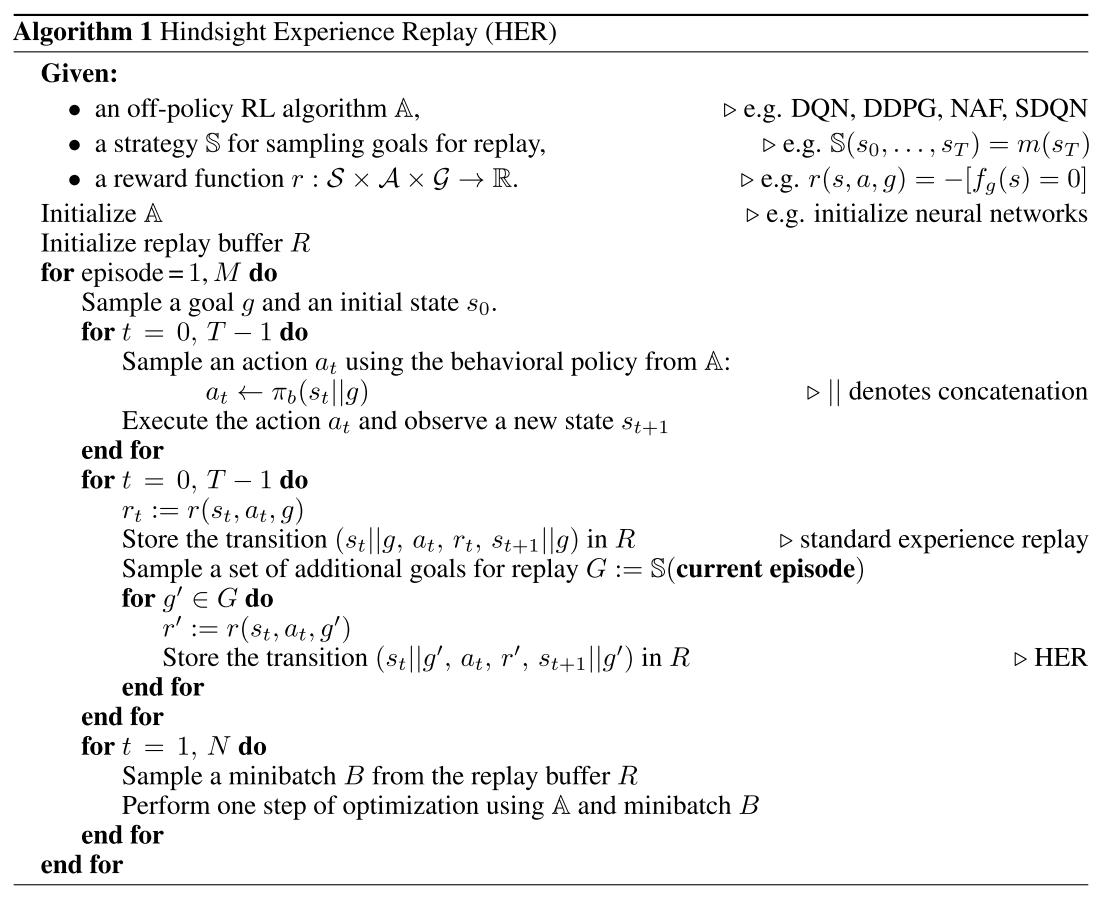
\includegraphics[scale=0.5]{her.png}
\caption{\label{Fig: her} Pseudocode of HER algorithm.}
\end{figure}
As shown in figure \ref{Fig: her}, the algorithm is as simple as effective: whenever we take an action during the training, we store the corresponding transition $(s_t \mid\mid g , a_t, r_t, s_{t+1}\mathbin\Vert g)$ in the replay buffer. Note that $s_t \mid \mid g$ denotes concatenation: when implementing Hindsight experience replay we're always giving concatenation of state and goal as input to both the actor (Policy) and critic (Q-value) networks. 
 After that, we sample from the transitions of the episode we've run a certain number (\textit{k}) of additional goals and we compute the reward function applied to each of this new goal and store in the replay buffer the corresponding transition . The hyperparameter \textit{k} can be seen as the ratio of data coming from HER to the replay buffer since it is the number of "HER" transitions stored in the replay buffer . The way we choose how to sample goals defines the strategy of the Hindisght experience replay method:
\begin{itemize}
\item \textit{future}  replays with k random states which come from the same episode as the transition being replayed and were observed after it
\item \textit{episode}  replays with k random states coming from the same episode as the transition being replayed
\item \textit{random}  replays with k random states encountered so far in the whole training procedure
\end{itemize}
In this work we tried do reproduce the results of the episodic strategy trying out different values of k. We also tried to implement a different strategy that is not mentioned in the original paper. In the paper is shown that all these strategies excluded the \textit{random} one are able to solve pushing task regardless the value of k.







\chapter{Experiments and Plots \label{exp}}

As previously  mentioned, our work consisted of implementing DDPG+HER in FetchPush-v1 environment trying to reproduce results obtained in \cite{her}. To implement our work we wrore the code in Python3 using TensorFlow 2.0. The code is structured in this way:

\begin{itemize}
\item a \textit{buffer.py} file in which is implemented the replay buffer in which the transitions are stored through the use of agent function \textit{remember()}. These transitions include state, new states, action, reward, a flag \textit{done} which indicates if the goal is reached and goal.In this file is also defined a function called \textit{sample\_buffer()} which is used in DDPG implementation for sampling a random minibatch of N transitions from the replay buffer.

\item a \textit{ddpg\_tf2.py} file in which all the parameters for the agent are defined and the DDPG algorithm is implemented. Here it is also initialized the target actor and target critic networks with the parameters reported in Table \ref{table}. Differently from \cite{her} in which it was used time-correlated OU noise, we used mean-zero Gaussian noise applied to the learned policy during exploration.
Here are defined a function for updating the network parameters that takes tau as input and implement the last stage of the pseudocode of DDPG algorithm, a remember function for storing the transitions, a function for saving and one for loading the models of the networks. In the file is also defined a function for choosing an action which takes as input the state and the goal, concatenate these as illustrated in the pseudocode of HER and gives it to the actor which computes the policy for choosing the action. The last function defined is the learning function, in which the critic network is updated by computing the target and applying the Mean Squared Error loss. While the actor network is updated by applying the ascent. 

\item a \textit{networks.py} file in which the actor and critic networks are created by following the conventional parameters used in this kind of tasks found on several papers regarding this argument (also reported in Table \ref{table}). The networks are created by using \textit{tensorflow.keras} and are formed by only dense layers with \textit{relu} as activation function, and a final critic dense output layer without activation function, and a final actor dense output layer with \textit{tanh} as activation function. Moreover the weights of the networks for training are saved in 2 files with extension \textit{.h5}, one for the critic network and one for the actor network. the critic network will return the Q function, while the actor network will return the policy $\mu$.



\item a \textit{main\_ddpg.py} file in which the training procedure is defined. In our implementation, this file contains the algorithm of Hindsight Experience Replay.

\end{itemize}

Most of the parameters we have used are taken from literature knowledge and from the papers cited in the Bibliography. In the following section the performed experiments are deeply explained. The following Table \ref{table} reports all the parameters used for all the experiments while the changed parameters will be illustrated in the specific section.
\\

\begin{table}[h]
\begin{center}
\begin{tabular}{|l|r|} 



\hline

\multicolumn{2}{|c|}{}\\
\multicolumn{2}{|c|}{\textbf{\Large            Parameters Table}}\\
\multicolumn{2}{|c|}{}\\

\hline

FC layers Critic 			& 2			\\
FC Critic dimensions		& 512		\\
Learning Rate Critic 		& 0.002		\\
FC layers Actor 			& 2			\\
FC Actor dimensions 		& 512		\\
Learning Rate Critic 		& 0.001		\\
Discount factor $\gamma$	& 0.99		\\
Update factor $\tau$		& 0.005		\\	%or 1?
Noise						& 0.1		\\
Replay Buffer dimension		& 1000000	\\

\hline
\end{tabular}
\end{center}
\caption{\label{table} Table of the parameters used for all the experiments}
\end{table}


\section{Training procedure and Plots}
This section will focus on experiments details and results. We will show the results we've obtained following the same algorithm and training procedures of \cite{her} along with a different one, that is more related to vanilla DDPG. When training following a basic version of DDPG  we also tried to implement a Hindsight experience replay strategy that is not presented in \cite{her} obtaining decent results.

\subsection{Episodic HER }
This subsection will focus on showing results obtained trying to reproduce \cite{her} results on training adopting the episodic strategy for hindsight experience replay. 

For the first groups of experiment we show different results obtained by changing the value of parameter k that establish the number of transitions taken for replaying. Following the procedure implemented in \cite{her} we performed these experiments to show that changing the value of \textit{k}, the system is always able to learn, as explained in \cite{her}. By following more strictly their training procedure (in detail what explained in Appendix A) we performed the training for 200 epochs, with each epoch formed by 50 cycle running 16 episodes. In this way each epochs contains $16 * 50=800$ episodes. During each episode, the agent choose actions according to policy $ \mu $ in 
$ 80 \%  $ of cases, whereas in the remaining cases the action is randomly sampled from the actions space . At the end of each cycle are performed 40 optimization steps in which the learning takes place and at the end of each episode HER is run and replace 	\textit{k} transitions in the replay buffer. In order to compute the rewards with the new substituted goals, we have computed the distance between the new goal, that is the box position reached during one random iteration of the episode, and the inital position of the box: if this distance was higher than the initial one between the box and the goal, then the transition was stored with a reward of $0$, otherwise it has been stored with -1. in the table \ref{exp1} are summarized some of the parameters used for the training. 
Success rate plots during training are shown in figures \ref{k4} \ref{k8} \ref{k16} \ref{k24}.  These plots show the best results we obtained among the many trials we attempted. In particular, we run the algorithm three times for each \textit{k}. We observed that most of the times the agent showed no learning at all. Observations about this behaviour are reported in the conlcusion subsection.

\begin{table}[h]
\begin{center}
\begin{tabular}{|l|r|} 



\hline

\multicolumn{2}{|c|}{}\\
\multicolumn{2}{|c|}{\textbf{\large    Parameters Table for the First Set of Experiments}}\\
\multicolumn{2}{|c|}{}\\

\hline

Batch Size 					& 128			\\
Number of Episodes			& 16			\\
Number of Cycles			& 50			\\
Number of Epochs			& 200			\\
k							& 4-8-16-24		\\
Number of episodes for test	& 100			\\


\hline
\end{tabular}
\end{center}
\caption{\label{exp2} Table of the specific parameters used for the second experiment with k equal to 8 random transitions.}
\end{table}

\begin{figure}[h!]
\begin{minipage}[b]{0.47\textwidth}
\centering
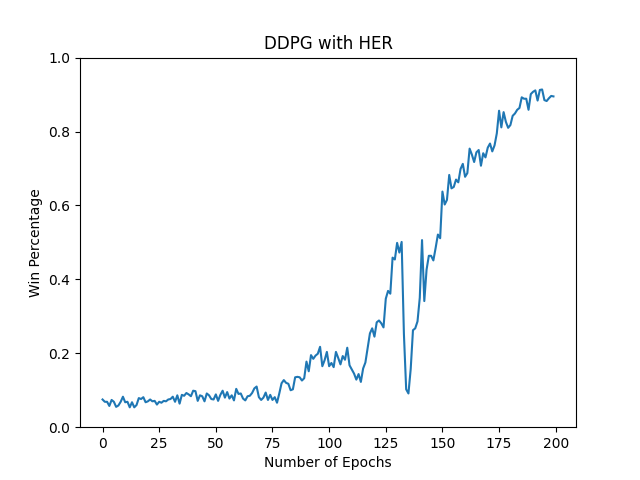
\includegraphics[width=\textwidth]{k4.png}
\caption{\label{k4}  $k=4$, maximum success rate reached 93\%.}
\end{minipage}
\hfill
\begin{minipage}[b]{0.47\textwidth}
\centering
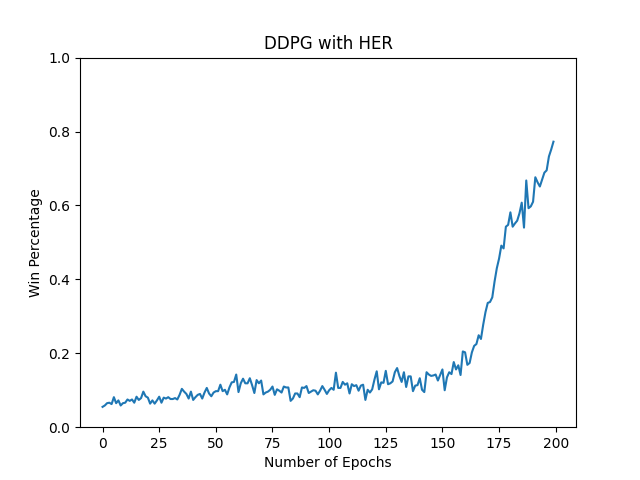
\includegraphics[width=\textwidth]{k8.png}
\caption{\label{k8} $k=8$, maximum success rate reached 78\%.}
\end{minipage}
\hfill
\begin{minipage}[b]{0.47\textwidth}
\centering
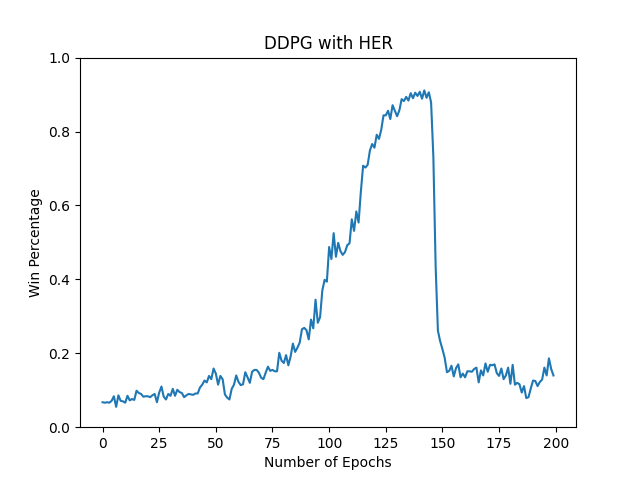
\includegraphics[width=\textwidth]{k16.png}
\caption{\label{k16}$k=16$, maximum success rate reached 92\%.}
\end{minipage}
\hfill
\begin{minipage}[b]{0.47\textwidth}
\centering
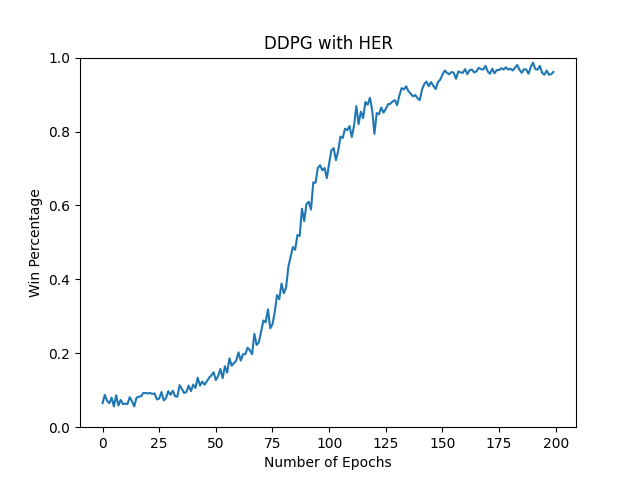
\includegraphics[width=\textwidth]{k24.png}
\caption{\label{k24} $k=24$, smaximum success rate reached 99\%.}
\end{minipage}
\end{figure}

\subsection{Initial/Final episodic HER}
After having achieved good results aiming to replicate the implementation in \cite{her}, we tried to implement a different HER strategy while following a different training procedure. For what regards the training method, we simply trained the algorithm for $50000$ episodes and in each episode we called the learning function everytime we chose an action. This is approach is more similar to the one reported in the pseudo-code of vailla DDPG \cite{ddpg}. The hindisght experience replay we implemented in this algorithm is a sort of episodic HER that instead of sampling \textit{k} random goals it takes \textit{k} first or final box positions encountered during the episode.  
In order to compute the reward for the new goals sampled, we assumed that if the distance between the goal and one of the inital (or final) position of the box was less than the distance computed taking into account one of the initial position and the initial position of the box the corresponding transition was stored with a reward of $0$.
As we can see from Figure \ref{img5} and Figure \ref{img6} the learning produces good results reaching a success around 93\% both in the case of finfal episodic HER and initial episodic HER However we have to mentioned that the training by considering the first 24 transitions is faster that the one that considers the last 24 transitions. For each of these two experiments we performed three trials and each time the system results to be able to learn. In the Table \ref{exp1} are reported the specific parameters used for the first two experiments.


\begin{figure}[h!]
\begin{minipage}[b]{0.47\textwidth}
\centering
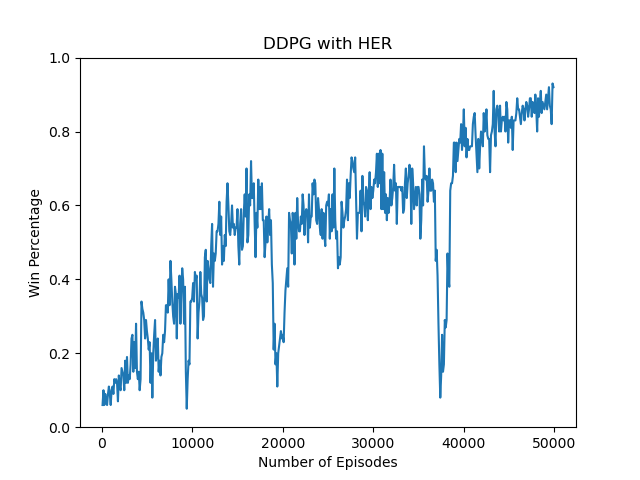
\includegraphics[width=\textwidth]{fetchpushnostroinitial.png}
\caption{\label{img5} Success rate for the 24 initial states taken, with normalized success rate equal to about 94\%.}
\end{minipage}
\hfill
\begin{minipage}[b]{0.47\textwidth}
\centering
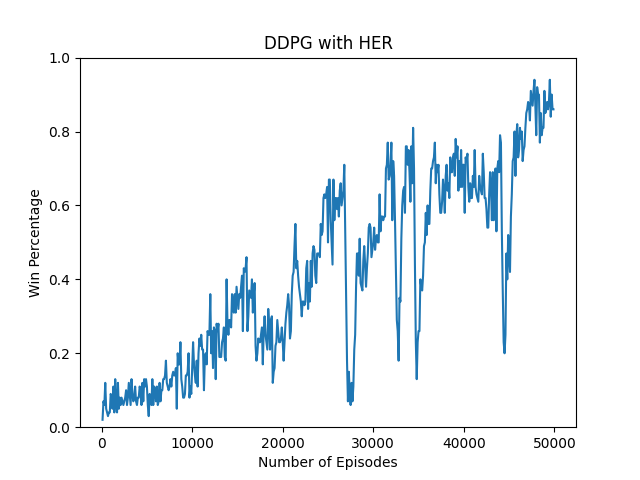
\includegraphics[width=\textwidth]{fetchpushnostrofinal.png}
\caption{\label{img6}Plots of the normalized success rate for the 24 last states taken, with normalized success rate equal to about 92\%.}
\end{minipage}
\end{figure}

\begin{table}[h]
\begin{center}
\begin{tabular}{|l|r|} 



\hline

\multicolumn{2}{|c|}{}\\
\multicolumn{2}{|c|}{\textbf{\large       Parameters Table for the Second Set of Experiments}}\\
\multicolumn{2}{|c|}{}\\

\hline

Batch Size 					& 64			\\
Number of episodes			& 50000			\\
k							& 24 (first and last)	\\


\hline
\end{tabular}
\end{center}
\caption{\label{exp1} Table of the specific parameters used for the second two experiments.}
\end{table}
 
\subsection{Conclusions}
At the end we managed to reproduce partially (mainly due to computational power issues) the results of \cite{her} and achieved good results when trying out new procedures and strategies. We already mentioned how several trainings showed no learning and we think that the reason behind this behaviour lies in the problem of vanishing gradient since we used as activation function for the actor network's last layer the hyperbolic tangent function $\tanh$. This problem could have been avoide by following what reported in \cite{her} :
"In order to prevent  tanh saturation and vanishing gradients we add the square of the their preactivations to the actor’s cost function". 




\begin{thebibliography}{}

\bibitem{multigoal}
Plappert, Matthias, et al. "Multi-goal reinforcement learning: Challenging robotics environments and request for research." arXiv preprint arXiv:1802.09464 (2018).

\bibitem{her}
Andrychowicz, Marcin, et al. "Hindsight experience replay." Advances in neural information processing systems. 2017.

\bibitem{ddpg}
Lillicrap, Timothy P., et al. "Continuous control with deep reinforcement learning." arXiv preprint arXiv:1509.02971 (2015).

\end{thebibliography}


\end{document}